\documentclass[a4paper, 12pt]{article}
\usepackage{graphicx}
\graphicspath{ {img/} }
\usepackage[hidelinks]{hyperref}
\usepackage{enumitem}
\begin{document}
	\title{Software speciifcation outline - Computer science forum.}
	\author{Group No. 2}
	\maketitle
	\section{Introduction}
		\subsection{Overview - Purpose of sytem}
		\par This document describes the specifications to which we designed our project around. We chose to create a Trinity Computer 
		Science centric forum that students and lecturers can use to communicate and share opinions and discuss module assignments and topics.
		\\\\Some parameters of the project are:
			\begin{enumerate}[label*=\arabic*.]
				\item Scope
				\begin{enumerate}[label*=\arabic*.]
					\item Computer Science centric, meaning there won’t be an option to 
					create new boards for different courses. Allowing this would increase 
					the difficulty of the project, and would rely heavily on lecturer/moderator participation to create each course’s board. 
					\item The scope of this project includes:
					\begin{enumerate}[label*=\arabic*.]
						\item Unique user names.
						\item Trinity email exclusive sign-up.
						\item Password protection.
						\item Topic creation.
						\item Replies to topics.
					\end{enumerate}
				\end{enumerate}

				\newpage
				\item Intended Audience
				\begin{enumerate}[label*=\arabic*.]
					\item We intend for this forum to be used by students of Computer Science, module demonstrators, lecturers and teaching assistants. Every user that signs up must have a valid TCD email address.
				\end{enumerate}
				\par The purpose that this project was created with was to give a place for students to discuss 
				problems or relevant topics with their coursemates. We felt that in a course like Computer Science, 
				an online communication board like this was a necessity to improve our communication with 
				our peers and to be able to learn from and help each other.
			\end{enumerate}
		\subsection{Abbreviations}
			\par Useful abbreviations for the following documents are:
			\begin{enumerate}[label*=\arabic*.]
				\item SCSS - School of Computer Science and Statistics.
				\item CS - Computer Science.
				\item CSB - Computer Science and Business.
				\item CSL - Computer Science and Language.
				\item HTML - HyperText Markup Language.
				\begin{enumerate}[label*=\arabic*.]
					\item Used as standard markup languge in creating websites.
				\end{enumerate}
				\item PHP - Personal Home Page.
				\begin{enumerate}[label*=\arabic*.]
					\item Used fpr web design and also as a general purpose programming language.
				\end{enumerate}
				\item UI - User Interface.
			\end{enumerate}
			\par References:
			\begin{enumerate}[label*=\arabic*.]
				\item VBulletin Community Forum help
				\begin{enumerate}[label*=\arabic*.]
					\item \url{http://www.vbulletin.com/forum/help?faq=vb3_board_usage#faq_vb3_forums_threads_posts}
				\end{enumerate}
				\item PHP Manual
				\begin{enumerate}[label*=\arabic*.]
					\item \url{http://php.net/manual/en/preface.php}
				\end{enumerate}
			\end{enumerate}
	\newpage
	\section{System Design}
		\subsection{Design Overview}
		\begin{enumerate}[label*=\arabic*.]
			\item The system is to be implemented in two parts
			\begin{enumerate}[label*=\arabic*.]
				\item \textbf{Back end implementation} - SQL Database.
				 \par This is where the forum’s actors are set out (Users, Unregistered Users and Moderators). It is also where all the data for forum users and forum posts are stored and called to from the Front end.
				 \item \textbf{Front-end implementation} - HTML + PHP.
				 \par This is what the user interacts with when using the CS forum. The front end is integrated with the back end functions to create new threads, new users, etc.
			\end{enumerate}
			\item The system is designed by integrating the front end aspects with the SQL database to 
			create a website that is constantly expanding through user input. The front end side of things 
			will load information from the database and display is according to the values and data 
			it finds, which means the front end will dynamically change for new threads created, and will 
			display new information when it updates such as post count for individual users.
			\item The system will be hosted on the Trinity KDEG machine, which is accessible to us 
			through the Trinity COMPSCI network. It is has a RAM of 1GB and 28GB of hard drive space, 
			which will be enough for us to create a more than sufficiently scaleable forum.
		\end{enumerate}
	\section{System Design Models}
		\subsection{System Context}
			\includegraphics[width=\textwidth]{systemContext.png}
		\subsection{UML Use Case}
			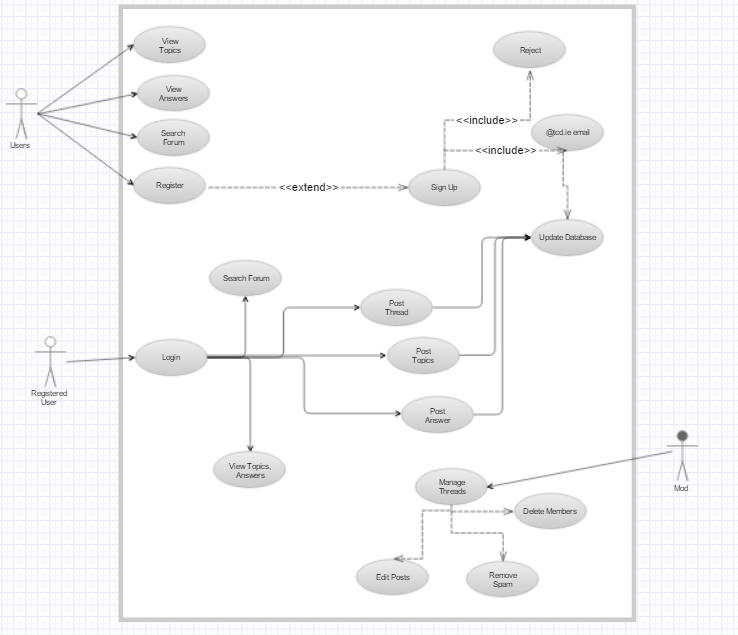
\includegraphics[width=\textwidth]{UMLUseCase.png}
	\section{System Architecture}
		\subsection{Class diagram}
			\includegraphics[width=\textwidth]{classDiagrams.png}
		\subsection{Sequence diagram}
			\includegraphics[width=\textwidth]{sequenceDiagram.png}
	\section{State diagrams}
		\subsection{Front end}
			\includegraphics[width=.9\textwidth,height=.9\textheight,keepaspectratio]{frontEnd.png}

		\subsection{Back end}
			\includegraphics[width=.9\textwidth,height=.9\textheight,keepaspectratio]{backEnd.png}

	\section{Activity diagram}
		\subsection{Logging in}
			\includegraphics[width=.9\textwidth,height=.9\textheight,keepaspectratio]{loggingIn.png}
	\section{Other diagrams}
		\subsection{Entity relationship diagram}
			\includegraphics[width=\textwidth]{entityRelationshipDiagram.png}
		\subsection{Functional dependency diagram}
			\includegraphics[width=\textwidth]{functionalDependency.png}
		\subsection{Relational schema}
			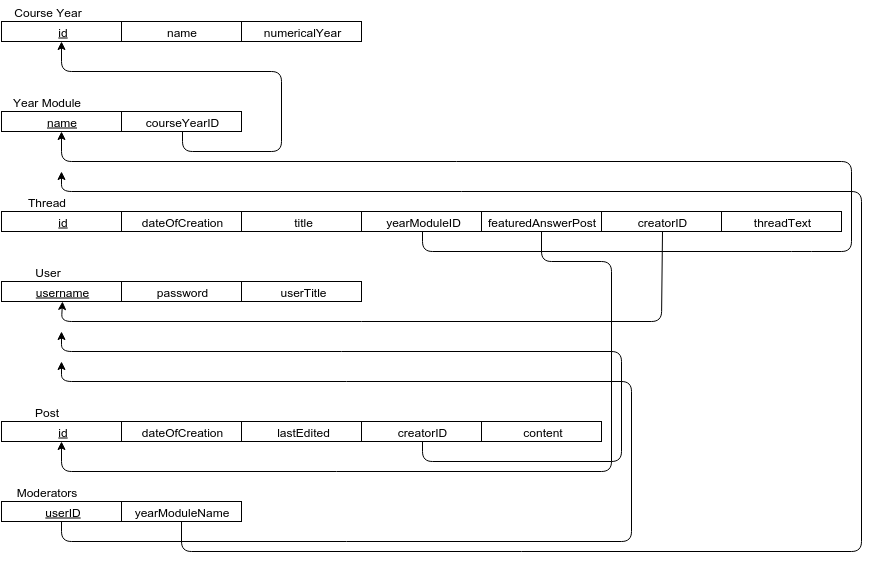
\includegraphics[width=\textwidth]{relationalSchema.png}

			
\end{document}
